%!TEX TS-program = xelatex
%!TEX encoding = UTF-8 Unicode

\documentclass[galley]{jtlu-article-2col} 
\usepackage{tabu}
\renewcommand\query[1]{\relax}

\graphicspath{{../Graphics/},{../../../../jtlugraphics/}}

%% ===== BEGIN ARTICLE DATA BLOCK - FILL IN THIS STUFF ==== %%
%% ===== JTLU publication and copyright info (required) === %%
\jtluissue{1}
\jtluvolume{7}								    	   
\jtluyear{2014}								   
\jtlurights{Firstname LastName}	 
\jtluid{nnn} 
\setcounter{page}{1} 

%% ===== ARTICLE TITLE (required), subtitle (optional) ==== %%
\title{Title in sentence case}
%\subtitle{Subtitle in sentence case}

%% ===== SHORT TITLE (required for page headers) ========== %%
\shorttitle{Short title}

%% ===== AUTHOR INFORMATION (required) ==================== %%             
%% Name, affiliation/institution, and email/contact for each
%% Add as many as necessary, separated by "\and":

\author{{\semibfsf Firstname LastName  } \\Organization  \thanks{title. email address}
  % \and {\bfseries } \\ 
  % \and {\bfseries } \\    
}% End authors

%% ===== END ARTICLE DATA BLOCK =========================== %%

\date{} % SET DATE TO NOTHING; NO DATE ON PAPERS

\hypersetup{%
			pdftitle={Title},
			pdfauthor={Firstname Lastname},
			pdfproducer={The Journal of Transport and Land Use vol. 7 no. 1 }
			pdfstartpage=1,
			colorlinks=true,
			linkcolor=NavyBlue,
			citecolor=PineGreen,
			urlcolor=BrickRed			
} % END HYPERSETUP


\begin{document}
\twocolumn[
\begin{@twocolumnfalse}
\maketitle
\begin{abstract}
Insert abstract here
\end{abstract}

\begin{keywords}
  Keyword 1; keyword 2; 
\end{keywords}
\end{@twocolumnfalse}
]
\saythanks

\section{Introduction}





\section{Section name}
\label{sec:section-name}



\subsection{Subsection heading}


%%%%%%%%%%
\begin{figure*}[htbp]
  \centering
  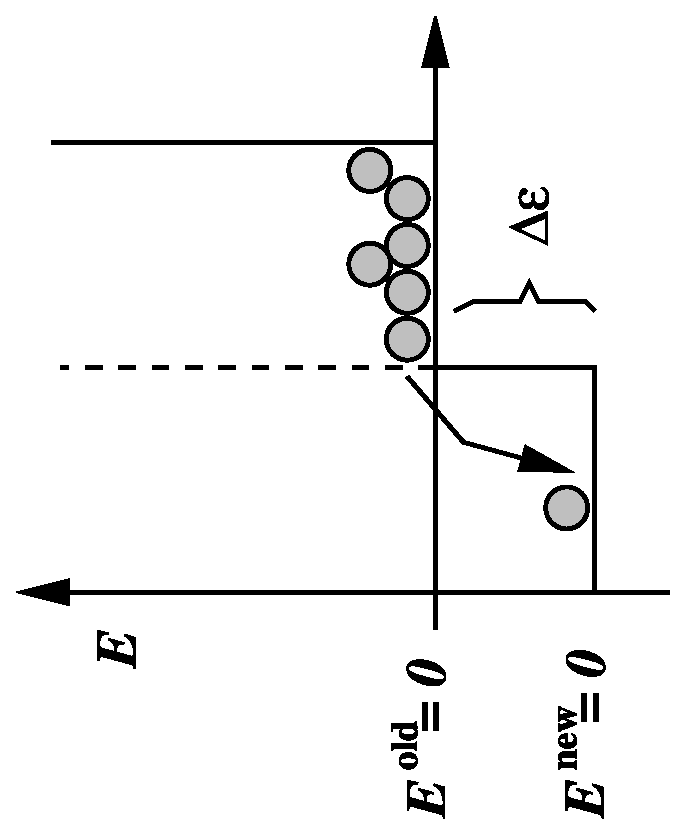
\includegraphics{fig1}
  \caption{Caption ...  }
  \label{fig:1}
\end{figure*}



\bibliographystyle{jtlu}
\bibliography{../Bib/filename}

\end{document}
